\chapter{Números Racionais}
%http://www.hypatiamat.com/apoiopdf/fracoes-I-hypatiamat.pdf


Os numeros racionais costuram apresentar uma grande dificuldade durante o aprendizado dos alunos. Isso se deve, em partes, a falta de abrangência com que os livros didáticos e/ou os professores no momento de se tratar desse tópico.

\section{Representações e Interpretações dos números racionais}

Em \cite{palhares2011complementos} as representações são classificadas entre icónicas \linebreak (ou pictóricas), em que se recorre a imagens e diagramas, ativas, em que se recorre a objetos, e simbólicas como as frações, números mistos, números decimais e as porcentagens (\%). Podem ter cunho discreto ou contínuo e podem ser modelos de área, comprimento, volume, tempo ou massa.

Alguns jogos que seriam muito bem empregados para abordar algumas dessas representações são o dominó de frações, que pode ser encontrado no blog \url{http://goo.gl/mcbyr0} e na dissertação que se encontra no link \url{http://goo.gl/XHCu6E}; o jogo da memória das frações, que pode ser encontrado em \url{http://goo.gl/z7t6Sy} para jogar online, e o applet em java para download no link \url{https://goo.gl/utAf0B} que possui diversas funcionalidades.

É dentre os Conteúdos Conteituais e Procedimentais dos PCNs que temos algumas das ``personalidades'' dos números racionais: parte-todo, quociente e razão. Esses três significados são acrescidos de ponto racional e operador por  \cite{onuchic2008diferentes}. 

Em \cite{palhares2011complementos} é feito uma revisão de algumas classificações diferentes que são mais profundamente abordadas na revisão bibliográfica feita no segundo capítulo da dissertação \linebreak \cite{rodriguesnumeros}.

\subsection{Exercícios e Problemas}
\begin{enumerate}
    \item Se a imagem seguinte 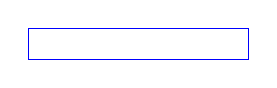
\begin{tikzpicture}[scale=.4]
  \draw[blue] (0,0) rectangle (7,1);
 \end{tikzpicture} representa $\dfrac{4}{5}$ de uma tira de papel, desenhe a tira completa.
 
 \item Investigue que tipo de frações geram dízimas finitas. Formule conjecturas e faça a prova.
 
 \item Observe a reta numérica onde estão marcados alguns números racionais representados pelas letras $A$, $B$, $C$ e $D$:
 
 \vspace{1cm}
 \begin{minipage}[h]{8cm}
 
 
     \begin{tikzpicture}[scale=5]

\draw[->] (-.3,0) -- (2.3,0);
\draw (0,.5pt) -- (0,-.5pt) node[anchor=north]{$0$};
\draw (1,.5pt) -- (1,-.5pt) node[anchor=north]{$1$};
\draw (2,.5pt) -- (2,-.5pt) node[anchor=north]{$2$};

\draw (1/3,.5pt) -- (1/3,-.5pt) node[anchor=north]{$A$};
\draw (5/6,.5pt) -- (5/6,-.5pt) node[anchor=north]{$B$};
\draw (1.5,.5pt) -- (1.5,-.5pt) node[anchor=north]{$C$};
\draw (2.05,.5pt) -- (2.05,-.5pt) node[anchor=north]{$D$};
\end{tikzpicture}
\end{minipage}
\vspace{1cm}

Qual a letra que melhor pode corresponder ao número que é o produto de $B$ por $C$? Marque na reta numérica o ponto que pode corresponder ao produto de $A$ por $C$. Marque também na reta numérica o ponto que pode corresponder à diferença entre $D$ e $C$.

\item Recorra às operações com frações para representar a parte sombreada da figura:

\begin{minipage}[h]{14cm}
\begin{center}
\begin{tikzpicture}[scale=1]
\draw (0,0) rectangle (4,2);
\draw (1,0) -- (1,2);
\draw (2,0) -- (2,2);
\draw (3,0) -- (3,2);

\draw (0,1) -- (1,1);

\draw[fill=grey!30] (0,1) rectangle (1,2);
\draw[fill=grey!30] (3,0) rectangle (4,8/7);

\draw (3,2/7) -- (4,2/7);
\draw (3,4/7) -- (4,4/7);
\draw (3,6/7) -- (4,6/7);
\draw (3,8/7) -- (4,8/7);
\draw (3,10/7) -- (4,10/7);
\draw (3,12/7) -- (4,12/7);
\end{tikzpicture}

\end{center}
\end{minipage}

\item Represente, recorrendo ao modelo de área, a seguinte expressão numérica:

$$\dfrac{1}{3}\times \dfrac{2}{5}+\dfrac{2}{3}\times \dfrac{1}{5}$$

\item Diga como procederia para calcular mentalmente os resultados das seguintes operações com números racionais:
\begin{multicols}{4}
\begin{enumerate}
    \item $2+\dfrac{1}{4}$
    \item $1-\dfrac{1}{4}$
    \item $3\times 3\dfrac{1}{5}$
    \item $3 \div \dfrac{1}{3}$
    \item $\dfrac{1}{2}+\dfrac{1}{4}$
    \item $\dfrac{1}{2}-\dfrac{1}{8}$
    \item $\dfrac{1}{2}\times \dfrac{3}{5}$
    \item $3\div\dfrac{3}{4}$
    \item $0,2+\dfrac{1}{5}$
    \item $0,5-\dfrac{1}{5}$
    \item $0,1\times \dfrac{1}{2}$
    \item $\dfrac{1}{3}\div 4$
    \item $\dfrac{2}{3}+5$
    \item $\dfrac{5}{3}-1$
    \item $\dfrac{3}{8}\times 8$
    \item $\dfrac{18}{16}\div\dfrac{9}{4}$
\end{enumerate}
\end{multicols}

Explique os raciocínios.

\section{Números Racionais em forma de Frações}

O conteúdo das frações é megaconceito pois engloba uma dezenas de outros. O seu trabalho desenvolve funções cognitivas que serão base para muitos outros conteúdos.

Algumas ideias chaves são:
\begin{enumerate}
    \item Uma fração pode ser maior que uma unidade;
    \item Duas frações podem ser equivalentes;
    \item Uma fração indica divisão em partes iguais;
    \item A fração conserva e recupera a unidade;
    \item Existe uma ordem entre as frações.
\end{enumerate}

Baseado em \cite{onuchic2008diferentes}, temos as seguintes personalidades dos números racionais:

\section{Ponto Racional}
Problemas que pedem para localizar números fracionários na reta numérica são ótimas oportunidades de trabalhar com essa personalidade. Todo número racional tem um ponto bem definido na reta e todo ponto racional da reta corresponde um número racional. 


\section{Quociente}
Essa personalidade normalmente é persebida quando um número de objetos precisa ser repartido igualmente num certo número de grupos. Esses objetos podem ter natureza contínua (pizza, barra) ou discreta (brinquedos).

Temos o dividendo e o divisor.A barra fracionária indica a função divisão. Essa personalidade é normalmente representado através da chave de divisão. Esse processo de aplica a diversos fenômenos como o processo de partição, extração, encolhimento e dedução.


\section{Fração}
Aqui temos a famosa relação parte-todo. Aqui interagem o numerador e o denominador. A barra fracionária apenas os separam.

Recomendo o jogo \textit{Loto }




\section{Operador}
Ocorre quando o múltiplicador (primeira parcela da multiplicação) é constituido por um número racinal. Por exemplo temos $\dfrac{3}{5}\times 15$.



Note que a barra fracionária indica a composição de operações divisão e multiplicação. 

Essa personalidade surge quando vamos encolher, esticar, reduzir ou ampliar algo.

\section{Razão}

Razão é uma comparação multiplicativa entre duas grandezas e não uma fração. Nelas se relacionam os termos antecedentes e consequêntes.

Essa personalidade é mais um conceito que liga diversos conteúdos como: regra de três, divisão em partes proporcionais, quantidades intensivas e extencivas, misturas, porcentagem, taxas, juros, descontos, escalas, estimativas populacionais, variação direta, variação inversa, razões trigonométricas, semelhança de triângulos, probabilidades, etc, além de ser base para o conceito de proporcionalidade.

\section{Proporcionalidade}
\end{enumerate}

%http://www.conhecer.org.br/enciclop/2015a/jogos%20matematicos.pdf

%http://arquivoabc.blogspot.com.br/p/fracoes.html
%http://www.sapientia.pucsp.br/tde_arquivos/3/TDE-2007-06-14T13:03:34Z-3492/Publico/dissertacao_wilson_roberto_rodrigues.pdf
%INCLUIR EXERCÍCIOS DOS COMPLEMENTOS E DO ARTIGO.

Livro: Física Conceitual
Capítulo: 12-Sólidos
Tópicos: Densidade (pg217), Mudanças de Escala (pg 223)

O que produz mais cascas, descascar 5kg de batatas grandes ou 5kg de batatas pequenas?

Área e volume não são diretamente proporcionais entre si.

\begin{enumerate}
    \item O que acontese ao volume de um pão que é esmagado? E à massa? E à densidade?
    \item O que é mais denso, algo que tenha uma densidade de $1.000 kg/m^3$, ou algo com densidade de $1g/cm^3$? Justifique sua resposta.
    \item O ósmio não é o átomo mais pesado encontrado na natureza. O que, então, explica que o ósmio seja a substância mais densa encontrada na Terra?
    \item O que tem maior densidade, uma pesada barra de ouro puro, ou um anel de ouro puro? Justifique sua resposta.
    \item A força do braço de uma pessoa depende do seu comprimento ou da área de sua seção transversal?
    \item Qual é o volume de um cubo de açucar com lado de 1 centímetro? Qual é a área da seção transversal desse cubo?
    \item O peso de uma pessoa depende mais do volume ou da área superficial da pele?
    \item Se as dimensões lineares de um certo objeto são dobradas, em quanto cresce sua área superficial? Em quanto cresce seu volume?
    \item Quando cresce o volume de um objeto, sua área superficial também cresce. Durante este crescimento, a razão dos metros quadrados para os metros cúbicos aumentam ou diminuem?
\end{enumerate}



